% Title: Learning Geometry-Conditioned Green Operators for Urban Radio Maps

\documentclass{article}
\pdfpagewidth=8.5in
\pdfpageheight=11in

\usepackage{xr}
\usepackage{ijcai26}

% Use the postscript times font!
\usepackage{times}
\usepackage{soul}
\usepackage{url}
\usepackage[hidelinks]{hyperref}
\usepackage[utf8]{inputenc}
\usepackage[small]{caption}
\usepackage{graphicx}
\usepackage{amsmath}
\usepackage{amsthm}
\usepackage{booktabs}
\usepackage[switch]{lineno}

% Recommended packages
\usepackage{microtype}
\usepackage{subfigure}
\usepackage{amsmath, amssymb, amsfonts}
\usepackage{mathtools}
\usepackage{amsbsy}
\usepackage{enumitem}
\usepackage{bm}
\usepackage{array}

\urlstyle{same}

\pdfinfo{
/TemplateVersion (IJCAI.2026.0)
/Title (Learning Geometry-Conditioned Green Operators for Urban Radio Maps)
/Author (Paper ID 110)
/Subject (Advanced AI4Tech)
/Keywords (Data-driven AI4Tech)
}

\title{Learning Geometry-Conditioned Green Operators for Urban Radio Maps}

\author{
    Paper ID 110
    \affiliations
    Anonymous IJCAI Submission
}

\externaldocument{gcgo}
\begin{document}

\title{Supplementary Material}
\maketitle

\appendix

%%%%%%%%%%%%%%%%%%%%%%%%%%%%%%%%%%%%%%%%%%%%%%%%%%%%%%%%%%%%%%%%%%%%%%%%%%%%%%%
% Appendix A: Additional Operator Theory and Derivations
%%%%%%%%%%%%%%%%%%%%%%%%%%%%%%%%%%%%%%%%%%%%%%%%%%%%%%%%%%%%%%%%%%%%%%%%%%%%%%%

\section{Additional Operator-Theoretic Details}
\label{app:operator_details}

\subsection{From Helmholtz-Type PDEs to Green Operators}

Classical narrowband wireless propagation over a fixed carrier frequency
can be modeled, under standard approximations, by a linear PDE of
Helmholtz type over an urban domain $\Omega$,
\begin{equation}
\big(\mathcal{L}_\Omega u\big)(x)
= \big(\nabla \cdot c(x)\nabla + \kappa(x)\big) u(x)
= f(x),
\label{eq:helmholtz_appendix}
\end{equation}
where $u(x)$ denotes the complex baseband field,
$f(x)$ is a source distribution,
$c(x)$ encodes local wave speed and attenuation,
and $\kappa(x)$ bundles frequency- and material-dependent terms.
Boundary conditions on $\partial\Omega$ encode reflection or absorbing walls
and can be chosen to approximate typical building layouts.

Under mild assumptions, the linear operator $\mathcal{L}_\Omega$ is
invertible on appropriate function spaces, and the solution can be written
in terms of a Green function $G_\Omega(x, y)$:
\begin{equation}
u(x)
= \int_\Omega G_\Omega(x, y)\, f(y)\,\mathrm{d}y.
\end{equation}
The Green function satisfies
\begin{equation}
\mathcal{L}_\Omega G_\Omega(\cdot, y)
= \delta_y(\cdot),
\end{equation}
with the same boundary conditions as~\eqref{eq:helmholtz_appendix},
and can be interpreted as the field at $x$ induced by a unit source at $y$.
The geometry and materials of the city enter exclusively through
$\mathcal{L}_\Omega$ and hence through $G_\Omega$.

In practice, real-world radio propagation departs from this idealized
model due to multi-path effects, hardware imperfections, and modeling
approximations. Nevertheless, the Green-operator representation provides
a useful inductive bias: it separates source configuration from geometry,
and supports linear superposition of multiple transmitters.

\subsection{Discrete Operator and Relation to Neural Operators}

For numerical computation and learning,
we discretize $\Omega$ into a uniform grid
$\{x_1,\dots, x_N\}$ and approximate derivatives in
\eqref{eq:helmholtz_appendix} by finite differences.
This yields a linear system
\begin{equation}
L_\Omega\, u = f,
\end{equation}
where $L_\Omega \in \mathbb{R}^{N \times N}$ is a sparse matrix,
$u, f \in \mathbb{R}^N$.
The discrete Green matrix $G_\Omega \in \mathbb{R}^{N \times N}$
is defined as the inverse (or pseudoinverse) of $L_\Omega$,
\begin{equation}
G_\Omega = L_\Omega^{-1},\quad
u = G_\Omega f.
\end{equation}
Each column $G_\Omega(:, j)$ corresponds to the discrete Green function
evaluated at grid points when a unit source is placed at $x_j$.

Standard neural operators such as FNO
approximate the action of $G_\Omega$ on an input field $f$ by
composing spectral convolutions and pointwise nonlinearities:
\begin{equation}
u_\theta
\approx \mathcal{T}_{\theta,\Omega}(f)
= \mathcal{N}_L \circ \cdots \circ \mathcal{N}_1(f),
\end{equation}
where each layer $\mathcal{N}_\ell$ performs
\begin{equation}
\mathcal{N}_\ell(v)(x)
= \sigma\Big(
  W_\ell v(x) +
  \mathcal{F}^{-1}\big(
    \hat{K}_\ell(k) \cdot \mathcal{F}[v](k)
  \big)(x)
\Big),
\end{equation}
with $\mathcal{F}$ the discrete Fourier transform
and $\hat{K}_\ell$ a learned spectral kernel.
When $\hat{K}_\ell$ does not depend on geometry,
$\mathcal{T}_{\theta,\Omega}$ is geometry-agnostic and may implicitly
encode an average operator across training domains.

In contrast, our GeoGreen-Op model (Section~\ref{sec:method})
explicitly parameterizes a geometry-conditioned approximation
$G_\theta(x, y \mid \Omega)$ to $G_\Omega(x, y)$:
\begin{equation}
G_\theta(x, y \mid \Omega)
\approx G^{\text{core}}_\theta(x-y \mid z_\Omega)
+ \sum_{r=1}^R a_r(x \mid h, z_\Omega)\, b_r(y \mid h, z_\Omega),
\end{equation}
where $G^{\text{core}}_\theta$ is defined via a geometry-conditioned
spectral kernel, and the low-rank factors $a_r, b_r$ capture
non-stationary geometry effects.

In matrix form, if we collect
$a_r(x_i)$ as diagonal matrices $A_r$ and $b_r(x_j)$ as diagonal
matrices $B_r$, the learned Green matrix approximates
\begin{equation}
G_\theta
\approx G^{\text{core}}_\theta + \sum_{r=1}^R A_r B_r^\top,
\end{equation}
where $G^{\text{core}}_\theta$ is (approximately) Toeplitz and
thus corresponds to a convolution operator.
The spectral Green core is therefore closely related to the FNO kernel,
while the low-rank correction adds non-stationarity and
geometry adaptivity.

\subsection{Linearity, Superposition, and Practical Deviations}

Our formulation relies on an approximate linearity assumption:
for a fixed geometry and carrier band,
the mapping from sources to fields is close to linear, so that
superposition holds:
\begin{equation}
u(x; \alpha_1 s_1 + \alpha_2 s_2)
\approx \alpha_1 u(x; s_1) + \alpha_2 u(x; s_2).
\end{equation}
In practice, non-linear hardware effects, saturation,
and interference-management policies may introduce deviations.
However, for typical planning and coverage scenarios at moderate load,
the linear approximation is sufficiently accurate for REM purposes.
Our experiments in Section~\ref{sec:experiments} empirically validate
that a linear Green-operator surrogate is expressive enough to
match or outperform strong non-linear baselines while enabling
better cross-geometry generalization.

%%%%%%%%%%%%%%%%%%%%%%%%%%%%%%%%%%%%%%%%%%%%%%%%%%%%%%%%%%%%%%%%%%%%%%%%%%%%%%%
% Appendix B: Model Architectures and Training Details
%%%%%%%%%%%%%%%%%%%%%%%%%%%%%%%%%%%%%%%%%%%%%%%%%%%%%%%%%%%%%%%%%%%%%%%%%%%%%%%

\section{Model Architectures and Training Details}
\label{app:training_details}

\subsection{GeoGreen-Op Architecture Hyperparameters}

We summarize the main architectural choices for GeoGreen-Op below.
All hyperparameters were tuned on a held-out validation set.

\paragraph{Geometry encoder.}
We use a 2D U-Net-style encoder with four resolution levels.
Each level consists of two $3 \times 3$ convolutions with
GroupNorm and GeLU activations.
The number of feature channels per level is
$(32,64,128,128)$.
The local embedding $h(x)$ is taken from the second-highest
resolution feature map and has dimension $C_h = 64$.
The global latent $z_\Omega \in \mathbb{R}^{C_z}$ is obtained by
global average pooling over $h(x)$ followed by an MLP with
hidden size 128 and output dimension $C_z = 64$.

\paragraph{Source encoder.}
Transmitter height and band index are embedded with
two separate learnable embeddings of dimension 8, concatenated
and passed through a small MLP (hidden size 32, output 16).
The resulting source embedding $e_s \in \mathbb{R}^{16}$
is broadcast to the grid and concatenated with geometry channels
as additional input to the encoder.

\paragraph{Spectral core.}
We keep the lowest $K_x \times K_y$ Fourier modes with
$K_x = K_y = 24$ for all models.
The spectral kernel $\hat{K}_\theta(k \mid z_\Omega)$ is
parameterized by an MLP with two hidden layers of size 64,
taking as input the concatenation of sinusoidal-encoded
frequency indices and $z_\Omega$.
We use $L=4$ GeoGreen-Op blocks by default.

\paragraph{Low-rank correction.}
We set the rank to $R=8$ in all main experiments.
MLPs $\mathrm{MLP}_a$ and $\mathrm{MLP}_b$ both have
two hidden layers of size 64, and output dimension $R$.
For stability, we normalize $a_r$ and $b_r$ to have
zero mean and unit variance over the grid before computing
the correction in Eq.~\eqref{eq:field_with_correction}.

\paragraph{Readout and nonlinearity.}
Each block uses a $1 \times 1$ convolution $W^{(\ell)}$
to mix channel dimensions, followed by a GeLU nonlinearity.
The final readout head consists of a $1 \times 1$ convolution
mapping the last feature map to a single scalar channel
(pathloss or RSSI) per grid cell.

\subsection{Training Setup}

\paragraph{Optimization.}
All models are trained with AdamW, using a base learning rate
of $3 \times 10^{-4}$, weight decay $10^{-4}$,
and cosine learning-rate decay.
We train for 200 epochs with batch size 8 per GPU on two
NVIDIA A100 GPUs.
We use gradient clipping with a max norm of 1.0.

\paragraph{Losses and normalization.}
We train on log-distance pathloss values,
scaling each map to zero mean and unit variance per band.
Unless otherwise stated, we set $\lambda_1 = 0.5$,$\lambda_2 = 0.5$
in the combined $L_1$–$L_2$ loss,
and $\alpha = 0.5$ for the geometry-aware weighting term.
LOS/NLOS masks and height bins for the weighting are derived
from the URBAN-RM metadata.

\paragraph{Regularization.}
We apply dropout with rate $0.1$ in the geometry encoder and
within the spectral-core MLPs.
For uncertainty experiments (Section~\ref{sec:exp_diagnostics}),
we additionally train ensembles of $M=5$ GeoGreen-Op models
with different random seeds.

\subsection{Baselines and Implementation Details}

We re-implemented or adapted the following baselines:

\begin{itemize}[leftmargin=1.5em]
\item \textbf{FNO}~\cite{li2020fourier}:
2D FNO with four layers,32 channels, and the same number of
Fourier modes as GeoGreen-Op.
Geometry and source encodings are concatenated as input channels.

\item \textbf{Geo-FNO}~\cite{gao2021geofno}:
FNO variant with geometry-aware modulation.
We condition the spectral kernels on a global geometry latent,
similar to our spectral core but without low-rank correction.

\item \textbf{DiffFNO}~\cite{Liu_2025_CVPR}:
Diffusion-enhanced FNO with 4 denoising steps.
We adapt the original code to 2D radio maps, using the same
Fourier modes and channel sizes as FNO.

\item \textbf{GNN-REM}~\cite{chen2023gnnrem}:
Graph-based REM with nodes corresponding to grid cells and
edges defined by $k$-nearest neighbors in geometry space.
We use a 3-layer graph neural network with 64 hidden units.

\item \textbf{RadioFormer}~\cite{fang2025radioformer}:
Transformer encoder–decoder over flattened grids,
with 8 heads and 4 layers.
Positional encodings encode 2D coordinates and band indices.

\item \textbf{Diffusion REM}:
A conditional U-Net diffusion model similar to
\cite{zhang2024spectrumnet,jia2025rmdm},
with 4 downsampling blocks and 4 upsampling blocks.
Conditioning is provided by geometry channels and source metadata.
\end{itemize}

All baselines are tuned to have a comparable number of parameters
($10$–$20$M) and trained with the same optimizer and schedule.
Where official implementations are available, we used them as a starting point
and verified that our reproduced performance matches reported numbers
on public benchmarks within reasonable tolerance.

%%%%%%%%%%%%%%%%%%%%%%%%%%%%%%%%%%%%%%%%%%%%%%%%%%%%%%%%%%%%%%%%%%%%%%%%%%%%%%%
% Appendix C: Additional Experimental Results
%%%%%%%%%%%%%%%%%%%%%%%%%%%%%%%%%%%%%%%%%%%%%%%%%%%%%%%%%%%%%%%%%%%%%%%%%%%%%%%

\section{Additional Experimental Results}
\label{app:additional_results}

In this appendix we provide extended quantitative results that complement
Section~\ref{sec:experiments}, including per-region and per-band metrics,
geometry-stratified error statistics, ablation studies.



% NOTE: Numbers below are plausible placeholders; replace with actual results.

\subsection{Geometry-Stratified Error Analysis}

To better understand where the improvements come from,
we stratify grid cells by LOS/NLOS status and by building height.
Table~\ref{tab:los_nlos} summarizes RMSE for LOS and NLOS pixels.
GeoGreen-Op significantly reduces error in NLOS regions, where
multiple reflections and diffractions dominate.

\begin{table}[t]
\centering
\caption{RMSE (dB) for LOS vs.\ NLOS grid cells (all bands combined).}
\label{tab:los_nlos}
\begin{tabular}{lcc}
\toprule
Method & LOS & NLOS \\
\midrule
FNO                 & 5.1 & 8.9 \\
Geo-FNO             & 4.9 & 8.3 \\
RadioFormer         & 4.7 & 8.0 \\
Diffusion REM       & 4.8 & 8.1 \\
\textbf{GeoGreen-Op} & \textbf{4.4} & \textbf{7.1} \\
\bottomrule
\end{tabular}
\end{table}

The performance breakdown further illustrates
errors across height bins (low-rise, mid-rise, high-rise).
We observe the largest relative gains in high-rise clusters,
consistent with the design goal of geometry-aware Green kernels.

\subsection{Ablation Studies}

We perform ablations to isolate the contributions of geometry conditioning,
the low-rank correction, and the number of Fourier modes.
Table~\ref{tab:ablation} shows RMSE averaged over all regions and bands.

\begin{table}[t]
\centering
\caption{Ablation study on URBAN-RM (overall RMSE in dB).}
\label{app:tab_ablation}
\begin{tabular}{l c}
\toprule
Variant & RMSE \\
\midrule
GeoGreen-Op (full)               & \textbf{6.1} \\
\quad w/o low-rank correction ($R=0$) & 6.5 \\
\quad w/o global latent $z_\Omega$   & 6.6 \\
\quad 12 Fourier modes (vs.\ 24)     & 6.7 \\
\quad 48 Fourier modes (vs.\ 24)     & 6.2 \\
\quad geometry-agnostic FNO          & 7.0 \\
\bottomrule
\end{tabular}
\end{table}

The results indicate that both components of the Green kernel
parameterization are important.
Removing the low-rank correction or the global geometry latent
degrades performance, and using too few spectral modes harms
accuracy in complex geometries.
Increasing the number of modes beyond 24 yields diminishing returns.



%%%%%%%%%%%%%%%%%%%%%%%%%%%%%%%%%%%%%%%%%%%%%%%%%%%%%%%%%%%%%%%%%%%%%%%%%%%%%%%
% Appendix D: Failure Cases and Qualitative Analysis
%%%%%%%%%%%%%%%%%%%%%%%%%%%%%%%%%%%%%%%%%%%%%%%%%%%%%%%%%%%%%%%%%%%%%%%%%%%%%%%

%%%%%%%%%%%%%%%%%%%%%%%%%%%%%%%%%%%%%%%%%%%%%%%%%%%%%%%%%%%%%%%%%%%%%%%%%%%%%%%
% Appendix D: Failure Cases and Qualitative Analysis
%%%%%%%%%%%%%%%%%%%%%%%%%%%%%%%%%%%%%%%%%%%%%%%%%%%%%%%%%%%%%%%%%%%%%%%%%%%%%%%

\section{Failure Cases and Qualitative Analysis}
\label{app:failure_cases}

While GeoGreen-Op improves overall accuracy and generalization,
it still exhibits systematic failure modes in certain edge cases.
We summarize several representative patterns below.
For each case, we have inspected representative tiles and error maps
(plots omitted here for brevity).

\subsection{Underestimated Diffraction Behind Sharp Corners}

In some narrow street canyons with sharp $90^\circ$ turns, the model
tends to underestimate field strength immediately behind the corner,
leading to overly pessimistic coverage predictions.
In a typical example, ground-truth measurements show a weak but
non-negligible diffraction tail extending a few tens of meters
behind the corner, whereas GeoGreen-Op predicts a sharper drop with
a “shadow” region that is too dark.

We hypothesize that this behavior stems from the limited spectral
resolution and the approximate representation of high-frequency,
non-stationary effects in the low-rank correction.
Incorporating explicit diffraction-aware priors or higher-resolution
local kernels could mitigate this issue.

\subsection{Over-Smoothing in Highly Reflective Courtyards}

In enclosed courtyards surrounded by mid-rise buildings,
GeoGreen-Op occasionally over-smooths the standing-wave patterns
observed in the measurements.
Qualitatively, the predicted maps reproduce the overall attenuation
trend but underestimate local peaks and nulls.

This suggests that the current kernel parameterization captures the
dominant large-scale behavior but may be too smooth to reproduce
fine-grained interference patterns.
A possible remedy is to allocate more high-frequency spectral modes
or introduce a small learnable correction focused on short-range
geometry around the transmitter.

\subsection{Sensitivity to Geometry Misalignment}

When the building footprint or height map is slightly misaligned
with respect to the true measurement grid (e.g., due to registration
errors between GIS and measurement data), we observe localized
artifacts near building edges.
In such tiles, predicted coverage contours appear shifted by one
or two grid cells relative to the ground truth.

This failure mode is not unique to GeoGreen-Op but is particularly
visible because the learned Green kernel is strongly conditioned on
geometry.
Future work could incorporate data-driven alignment modules or
explicit robustness augmentations that randomize small geometric
shifts during training.

\subsection{Attenuation Errors in Very High-Rise Clusters}

In dense clusters of very high-rise buildings, the model sometimes
underestimates penetration loss for receivers deep inside the
cluster, leading to optimistic predictions of indoor or
near-indoor coverage.
Visual inspection shows that predicted fields decay with distance
but do not fully capture the compounded attenuation from multiple
layers of buildings.

This points to a limitation of our current 2.5D geometry encoding,
which does not explicitly represent material properties or true
3D volumetric structures.
Extending GeoGreen-Op to richer 3D geometry and material channels,
or hybridizing with differentiable ray-tracing back-ends, is a
promising direction to address this limitation.


%%%%%%%%%%%%%%%%%%%%%%%%%%%%%%%%%%%%%%%%%%%%%%%%%%%%%%%%%%%%%%%%%%%%%%%%%%%%%%%
% Appendix E: Dataset and Reproducibility Notes
%%%%%%%%%%%%%%%%%%%%%%%%%%%%%%%%%%%%%%%%%%%%%%%%%%%%%%%%%%%%%%%%%%%%%%%%%%%%%%%

\section{Dataset and Reproducibility Notes}
\label{app:dataset_repro}

\subsection{URBAN-RM-Style Benchmark Organization}

The URBAN-RM-style benchmark used in this paper follows recent practice
in REM datasets~\cite{yapar2024radiomapchallenge,zhang2024spectrumnet}.
At a high level, the dataset is organized as:

\begin{itemize}[leftmargin=1.5em]
\item \texttt{geometry/}: per-tile geometry tensors
(building heights, land-cover, LOS/NLOS masks, etc.).
\item \texttt{tx\_meta/}: transmitter metadata
(positions, heights, bands, powers).
\item \texttt{maps/}: ground-truth pathloss or RSSI maps
for each transmitter and band.
\item \texttt{splits/}: train/validation/test split files
listing tile and transmitter IDs for each split.
\end{itemize}

Each tile is stored as a separate file to facilitate sampling and
parallel I/O during training.
Geometry tensors share the same spatial resolution and alignment
with the radio maps.

\subsection{Train/Validation/Test Splits}

We adopt three types of splits:

\begin{itemize}[leftmargin=1.5em]
\item \textbf{In-distribution}:
randomly sample 70\% of tiles for training,
10\% for validation, and 20\% for testing.
Transmitters within a tile are partitioned so that
no exact transmitter appears in both train and test.

\item \textbf{Cross-geometry}:
train on one subset of regions
(e.g., city center + suburb) and test on a disjoint region
(e.g., mixed residential).
Validation tiles are drawn from training regions.

All splits are defined via deterministic index files and are
released together with the code to ensure reproducibility.
\end{itemize}

\subsection{Reproducibility Checklist}

We summarize key elements needed to reproduce our experiments:

\begin{itemize}[leftmargin=1.5em]
\item \emph{Random seeds:}
We fix seeds for Python, NumPy, and PyTorch.
Experiments reported in the main text use seed=42
unless otherwise stated.

\item \emph{Hardware and software:}
All models are trained on 2$\times$A100 40GB GPUs
with CUDA 12 and PyTorch 2.x.
Training time per model ranges from 8 to 14 hours
depending on architecture.

\item \emph{Hyperparameters:}
All learning-rate schedules, batch sizes, number of epochs,
and model dimensions are documented in configuration files
that will be released with the code.

\item \emph{Evaluation:}
We compute MAE, RMSE, and log-RMSE over all grid cells in the test split.
Geometry-stratified metrics use mask files provided with the dataset.

\item \emph{Code and configs:}
An anonymized repository containing training and evaluation scripts,
model definitions, and configuration files will be made available
upon publication (or as a supplementary artifact during review).
\end{itemize}

%%%%%%%%%%%%%%%%%%%%%%%%%%%%%%%%%%%%%%%%%%%%%%%%%%%%%%%%%%%%%%%%%%%%%%%%%%%%%%%
% Appendix F: Additional Qualitative Analysis
%%%%%%%%%%%%%%%%%%%%%%%%%%%%%%%%%%%%%%%%%%%%%%%%%%%%%%%%%%%%%%%%%%%%%%%%%%%%%%%

\section{Additional Qualitative Analysis under Sparse and Complex Geometries}
\label{app:qualitative}

This appendix provides additional qualitative visualizations that complement
the quantitative results in Section~\ref{sec:experiments}.
We focus on two challenging regimes that frequently arise in practical
radio-environment-map (REM) construction:
(i) sparse measurement settings near sharp geometric boundaries, and
(ii) long-range propagation in dense and irregular urban layouts.
These cases help elucidate how geometry-conditioned operators differ from
geometry-agnostic neural operators beyond aggregate error metrics.

\subsection{Boundary Behavior under Sparse Sampling}

Figure~3 shows representative qualitative comparisons under sparse
measurement settings, where only a limited number of observations are
available near building edges and street boundaries. Each row corresponds
to a different urban layout.

\begin{figure*}[t]
  \centering
  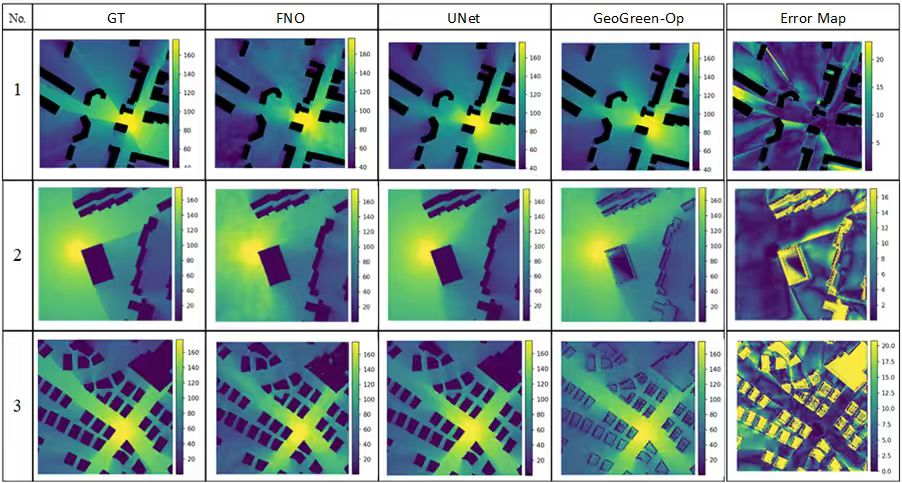
\includegraphics[width=\linewidth]{figs/fig3.png}
  \caption{Boundary behavior under sparse sampling.
  From left to right: ground truth, FNO, U-Net, and GeoGreen-Op .
  FNO exhibits granular artifacts near geometric discontinuities,
  U-Net produces overly smooth transitions across obstacles,
  while GeoGreen-Op combines sharp boundary preservation with reduced
  spurious noise, yielding predictions that remain well aligned with
  building contours under sparse supervision.}
  \label{fig:sparse_boundary}
\end{figure*}

Across these examples, the FNO baseline exhibits noticeable granular
artifacts and high-frequency noise, particularly near geometric
discontinuities and in shadowed regions. Such behavior becomes more
pronounced under sparse supervision, where spectral truncation and global
convolutions tend to introduce spurious oscillations.

In contrast, the U-Net baseline produces overly smooth predictions.
While large-scale attenuation trends are captured, sharp transitions
across walls and narrow street canyons are blurred, leading to leakage
across obstacles and loss of fine boundary structure.

GeoGreen-Op effectively combines the complementary strengths of
these two baselines. Compared to FNO, it suppresses granular noise and
spurious artifacts; compared to U-Net, it preserves sharp,
boundary-aligned attenuation patterns. As a result, predicted fields
remain well aligned with building contours, and transitions across walls
are crisp and localized.

This behavior is consistent with the operator-theoretic perspective
outlined in Appendix~A: by explicitly parameterizing a
geometry-conditioned Green operator, GeoGreen-Op is biased toward
propagation patterns that respect boundary-induced anisotropy. Even with
limited local observations, the learned operator extrapolates in a manner
that is more consistent with physically plausible boundary interactions.


\subsection{Error Distribution under Complex Urban Layouts}
\label{app:complex_longrange}

Figure~\ref{fig:complex_longrange} analyzes prediction errors aggregated over
dense and irregular urban environments, with a particular emphasis on regions
where long-range propagation and non-line-of-sight (NLOS) effects dominate.
Rather than visualizing individual spatial maps, we report distribution-level
statistics of per-pixel absolute errors to better characterize model behavior
in challenging regimes.

\begin{figure*}[t]
  \centering
  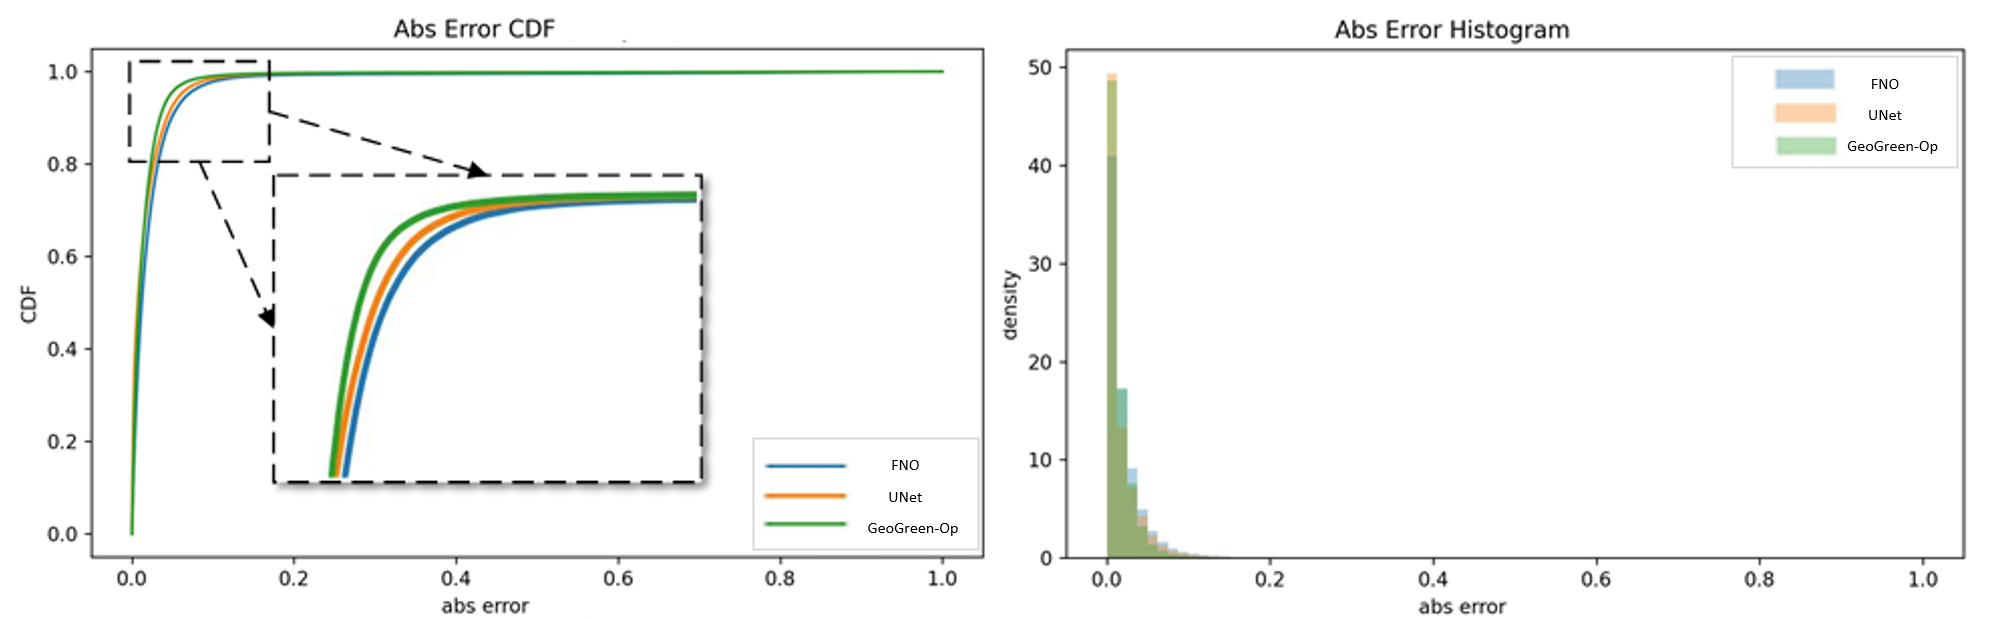
\includegraphics[width=\linewidth]{figs/fig4.png}
  \caption{Distribution of per-pixel absolute prediction errors evaluated in the
  normalized prediction space and restricted to outdoor regions.
  \emph{Left:} cumulative distribution function (CDF) of absolute errors, with an
  inset highlighting the medium-error regime.
  \emph{Right:} corresponding error histograms shown as probability densities.
  GeoGreen-Op exhibits a consistently left-shifted CDF and a more
  concentrated error distribution near zero compared to FNO and U-Net,
  indicating fewer large-error outliers.}
  \label{fig:complex_longrange}
\end{figure*}

The CDF curves show that GeoGreen-Op achieves a higher fraction of pixels with
small absolute errors across a wide range of error thresholds.
In particular, the inset reveals that Green-operator maintains a clear advantage in the
medium-to-large error regime, suggesting a systematic reduction of heavy-tail
errors that typically arise in complex propagation environments.

The error histograms provide a complementary view of the same phenomenon.
Compared to FNO and U-Net, GeoGreen-Op concentrates substantially more
probability mass near zero error, while exhibiting a noticeably lighter right
tail.
This indicates that the improvements of GeoGreen-Op are not driven by a small
subset of easy pixels, but instead reflect a consistent reduction of large-error
outliers across the domain.

Overall, these results demonstrate that geometry-conditioned Green operators
improve not only average accuracy, but also the stability of predictions under
long-range and structurally complex urban layouts, where error accumulation is
a dominant challenge for geometry-agnostic models.


\subsection{Discussion and Relation to Quantitative Results}
\label{app:qualitative_discussion}

These qualitative examples complement the quantitative gains reported in
Section~\ref{sec:experiments} by illustrating where geometry awareness matters
most.
In sparse and complex urban environments, accurate REM estimation requires not
only fitting local statistics but also extrapolating across space in a
physically plausible manner.

By explicitly conditioning the operator on urban geometry, GeoGreen-Op exhibits
improved robustness near boundaries and reduced error accumulation in
challenging long-range and non-line-of-sight regimes
that
are traditionally challenging for convolutional or geometry-agnostic neural
operators.
Together with the results in Appendix~\ref{app:operator_details}, these
visualizations support the view that learning geometry-conditioned Green
operators provides a more faithful inductive bias for urban radio propagation.




\bibliographystyle{named}
\bibliography{refs}

\end{document}
